%!TEX program = xelatex
% 完整编译: xelatex -> biber/bibtex -> xelatex -> xelatex
\documentclass[lang=cn,11pt,a4paper]{elegantpaper}

\title{centered.h文档说明}
\author{Haochen Huang}

\version{4.02test}
\date{\zhtoday}


% 本文档命令
\usepackage{array}

\begin{document}

\maketitle
\tableofcontents

\begin{abstract}
本文为basilisk的头文件center.h的说明文档,在阅读时请结合poisson.h、bcg.h、viscosity.h等说明头文件。\par
2.02版本更新,全面更正之前错误,添加附录解释加速度项更新及Basilisk执行规则,添加程序示意图,更新理论部分,更新程序注释。\par
3.02版本更新确认了Basilisk中event的继承顺序,修改部分笔误\par
4.02版本重新确认并更正了此前在理论部分出现的重大错误,并借由此从更深刻的角度重新理解相关求解器

\end{abstract}


\section{理论背景}

\subsection{文件目的}
本文件的目的是求解不可压$NS$方程,文件相关离散格式请见\cite{popinet2003gerris}\cite{popinet_accurate_2009}:
\begin{gather}\label{equ:bukeyans}
    \frac{\partial \mathbf{u}}{\partial t}+\nabla\cdot(\mathbf{u}\otimes\mathbf{u})= \frac{1}{\rho}[-\nabla p+\nabla\cdot(2\mu\mathbf{D})]+\mathbf{a}\\
    \nabla \cdot\mathbf{u} = 0
\end{gather}

\subsection{理论求解综述}
本求解器使用$Approximate \,Projection \,Method$(下称$APM$)对不可压缩$NS$方程进行求解:\par
对原方程\ref{equ:bukeyans}进行离散有:
\begin{equation}\label{equ:discretization}
        \begin{aligned}
        \rho^{n+\frac{1}{2}}\frac{\mathbf{u}^{n+1} - \mathbf{u}^{n}}{\Delta t}+\nabla\cdot(\mathbf{u}^{n+\frac{1}{2}}\otimes\mathbf{u}^{n+\frac{1}{2}})=  \nabla \cdot [\mu^{n+\frac{1}{2}}(\mathbf{D^{n+1}}+\mathbf{D^n})]+ [\mathbf{a}^{n+1}-\nabla p^{n+1}]
    \end{aligned}
\end{equation}
理论上$\mathbf{u}^{n+1},\mathbf{u}^{n}$满足无散条件;
式\ref{equ:discretization}中已知条件为$\mathbf{u}^n,\nabla p^{n}$而待解项为$\mathbf{u}^{n+1},\nabla p^{n+1}$。\par
与$MAC$相似\cite{harlow1965numerical},该方法的第一步都为计算不满足无散条件的中间步$ \mathbf{u} ^*$:
\begin{equation}\label{yucebu}
    \rho^{n+\frac{1}{2}}\frac{\mathbf{u}^* - \mathbf{u}^{n}}{\Delta t}+\nabla\cdot(\mathbf{u}^{n+\frac{1}{2}}\otimes\mathbf{u}^{n+\frac{1}{2}})= \nabla \cdot [2\mu^{n+\frac{1}{2}}\mathbf{D^*}]+ \mathbf{a}^{n}-\nabla p^{n}
\end{equation}
注意$\mathbf{u^*}$并不需要满足无散条件。此处求解器选择$APM$的$pressure\, form$\cite{drikakis2005high},即在相应的投影之前需要对$ \mathbf{u} ^*$进行相应的处理
\begin{equation}\label{equ:poisson}
    \mathbf{u}^{n+1} = \mathscr{P}( \mathbf{u}^* + \frac{\Delta t}{\rho^{n+\frac{1}{2}}}( -\mathbf{a}^{n} + p^{n}))
\end{equation}
其中$\mathscr{P}$代表投影算子;两式中扩散项之差作为改方法在时间上的误差记$\epsilon$有
\begin{equation}
    \epsilon = (\Delta t)^2\mathscr{L}(\frac{1}{\rho}\mathscr{G}(\frac{\partial p}{\partial t}))+\frac{1}{2}\Delta t\mathscr{L}(\frac{\partial \mathbf{u}}{\partial t})
\end{equation}
$\mathscr{L},\mathscr{G}$分别是拉普拉斯与梯度算子。\par
\textbf{接下来依顺序求解方程\ref{yucebu}}\par
首先启用bcg.h处理对流项,bcg.h得目的为求解方程:
\begin{equation}\label{equ:duiliu}
    u^{**}=u^n-\Delta t \mathbf{A}
\end{equation}
其中$\mathbf{A}$就是$\nabla\cdot(\mathbf{u}^{n+\frac{1}{2}}\otimes\mathbf{u}^{n+\frac{1}{2}})$的bcg离散格式,由此我们就可以将对流项加入到非定常项中,\ref{yucebu}变为:
\begin{equation}\label{equ:vis}
    \rho_{n+\frac{1}{2}}\frac{\mathbf{u}^* - \mathbf{u}^{**}}{\Delta t}= \nabla \cdot [2\mu^{n+\frac{1}{2}}\mathbf{D^*}]+[\mathbf{a}^{n}-\nabla p^{n}]
\end{equation}
再将非扩散项的源项汇入非定常项,最后得到
\begin{equation}\label{equ:kuosan}
    \rho_{n+\frac{1}{2}}\frac{\mathbf{u}^* - \mathbf{u}^{***}}{\Delta t}= \nabla \cdot [2\mu^{n+\frac{1}{2}}\mathbf{D^*}]
\end{equation}
其中
\begin{equation}\label{equ:yuanxiangjiazai}
    \mathbf{u}^{***} = u^{**}+\frac{\Delta t}{\rho_{n+\frac{1}{2}}}[\mathbf{a}^{n}-\nabla p^{n}]
\end{equation}
由viscosity.h求解该方程,得到$\mathbf{u^*}$。再由方程\ref{equ:poisson}填补加速项与已知压力梯度项$\nabla p^{n}$得$u^*_{new}$
\begin{equation}\label{equ:sudugengxin}
    \mathbf{u^*_{new}}=\mathbf{u^*}-\frac{\Delta t}{\rho_{n+\frac{1}{2}}}(-\nabla p^{n}+\mathbf{a^{n}}-\mathbf{a^{n+1}}) = \mathbf{u}^{n+1} + \nabla p^{n+ 1}
\end{equation}
又因为$\mathbf{u}^{n+1}$满足无散条件,即可得到poisson方程
\begin{equation}
     \nabla\mathbf{u^*_{new}}=\Delta p^{n+1}
\end{equation}
由此更新速度$\mathbf{u}^{n+1}$以及速度梯度项$\nabla p^{n+1}$

\subsection{$APM$与$EPM$}
如前文所述,本求解器算法为近似投影法($APM$)而并非标准投影法($EPM$),二者主要区别在与对拉普拉斯算子$\mathscr{L}$的构造以及最后结果是否满足无散条件。将\ref{equ:bukeyans}改写为(忽略加速度项):
\begin{equation}
    \frac{\partial \mathbf{u}}{\partial t}+\frac{1}{\rho}\nabla p= \frac{1}{\rho}[\nabla\cdot(2\mu\mathbf{D})]-\nabla\cdot(\mathbf{u}\otimes\mathbf{u})
\end{equation}
观察到方程右端为连续向量场,依照定义对其施加投影算子$\mathscr{P}$有
\begin{equation}
    \frac{\partial \mathbf{u}}{\partial t}=\mathscr{P} (\frac{1}{\rho}[\nabla\cdot(2\mu\mathbf{D})]-\nabla\cdot(\mathbf{u}\otimes\mathbf{u}))
\end{equation}
使用分布法实现该投影算子,即求解方程\ref{equ:discretization}首先得到$\mathbf{u}^*$,再通过$possion$求解器更新速度项与压力梯度项,即:
\begin{equation}\label{equ:renew}
    \mathscr{D}\mathscr{G}\phi =\mathscr{L} \phi= \mathscr{D}\mathbf{V}
\end{equation}
其中$\mathscr{D},\mathscr{G},\mathscr{L}$分别代表散度算子,梯度算子,拉普拉斯算子。$EPM$与$APM$之间的差别就在于$\mathscr{L}$的构建,对于$EPM$,$\mathscr{L}_{EPM}= \mathscr{D} \mathscr{G}$即拉普拉斯算子并不单独存在而是由两离散的算子计算合成的,然而这样构成的拉普拉斯算子在实际的操作尤其是自适应网格等复杂网格中很难实现,是故诞生了$APM$,即单独定义标准的$\mathscr{L}$,而往往$\mathscr{L}_{APM}\neq \mathscr{D} \mathscr{G}$,从而导致计算结果$ \mathbf{u}^{n+1}$并不能满足严格的无散条件,而是对标准无散速度的二阶近似,近似投影法$APM$也因此得名。\par
$\phi, \mathbf{V}$则分别代表余项以及相应的无散化矢量,根据不同需要$ \mathbf{V}$有不同选择\cite{almgren2000approximate},在$EPM$中$ \mathbf{V}$的选择并不影响最终结果,然而对于$APM$,$ \mathbf{V}$的选择会极大的影响最终的误差积累。本求解器在此处选取的形式为
\begin{equation}
    \mathbf{V} = \mathbf{u}^* + \frac{\Delta t}{\rho^{n + \frac{1}{2}}}(\nabla p^n) 
\end{equation}
根据\cite{almgren2000approximate},此种模式在$APM$中相较其他选择具有最强的稳定性。
\section{源代码解析}
\subsection{代码构成及结构简介}
同上文原理,代码共有五部分:
\begin{enumerate}
    \item 初始边界设置,初始条件设置\ref{sec:fundemantel}
    \item 对流项处理\ref{sec:advection}
    \item 扩散项处理\ref{sec:diffusion}
    \item 加速度更新\ref{sec:projection}
    \item 速度投影与压力梯度更新
\end{enumerate}
其中最后两部分合并编写,整体求解器示意图如下:
\begin{figure}[h]
  \centering
  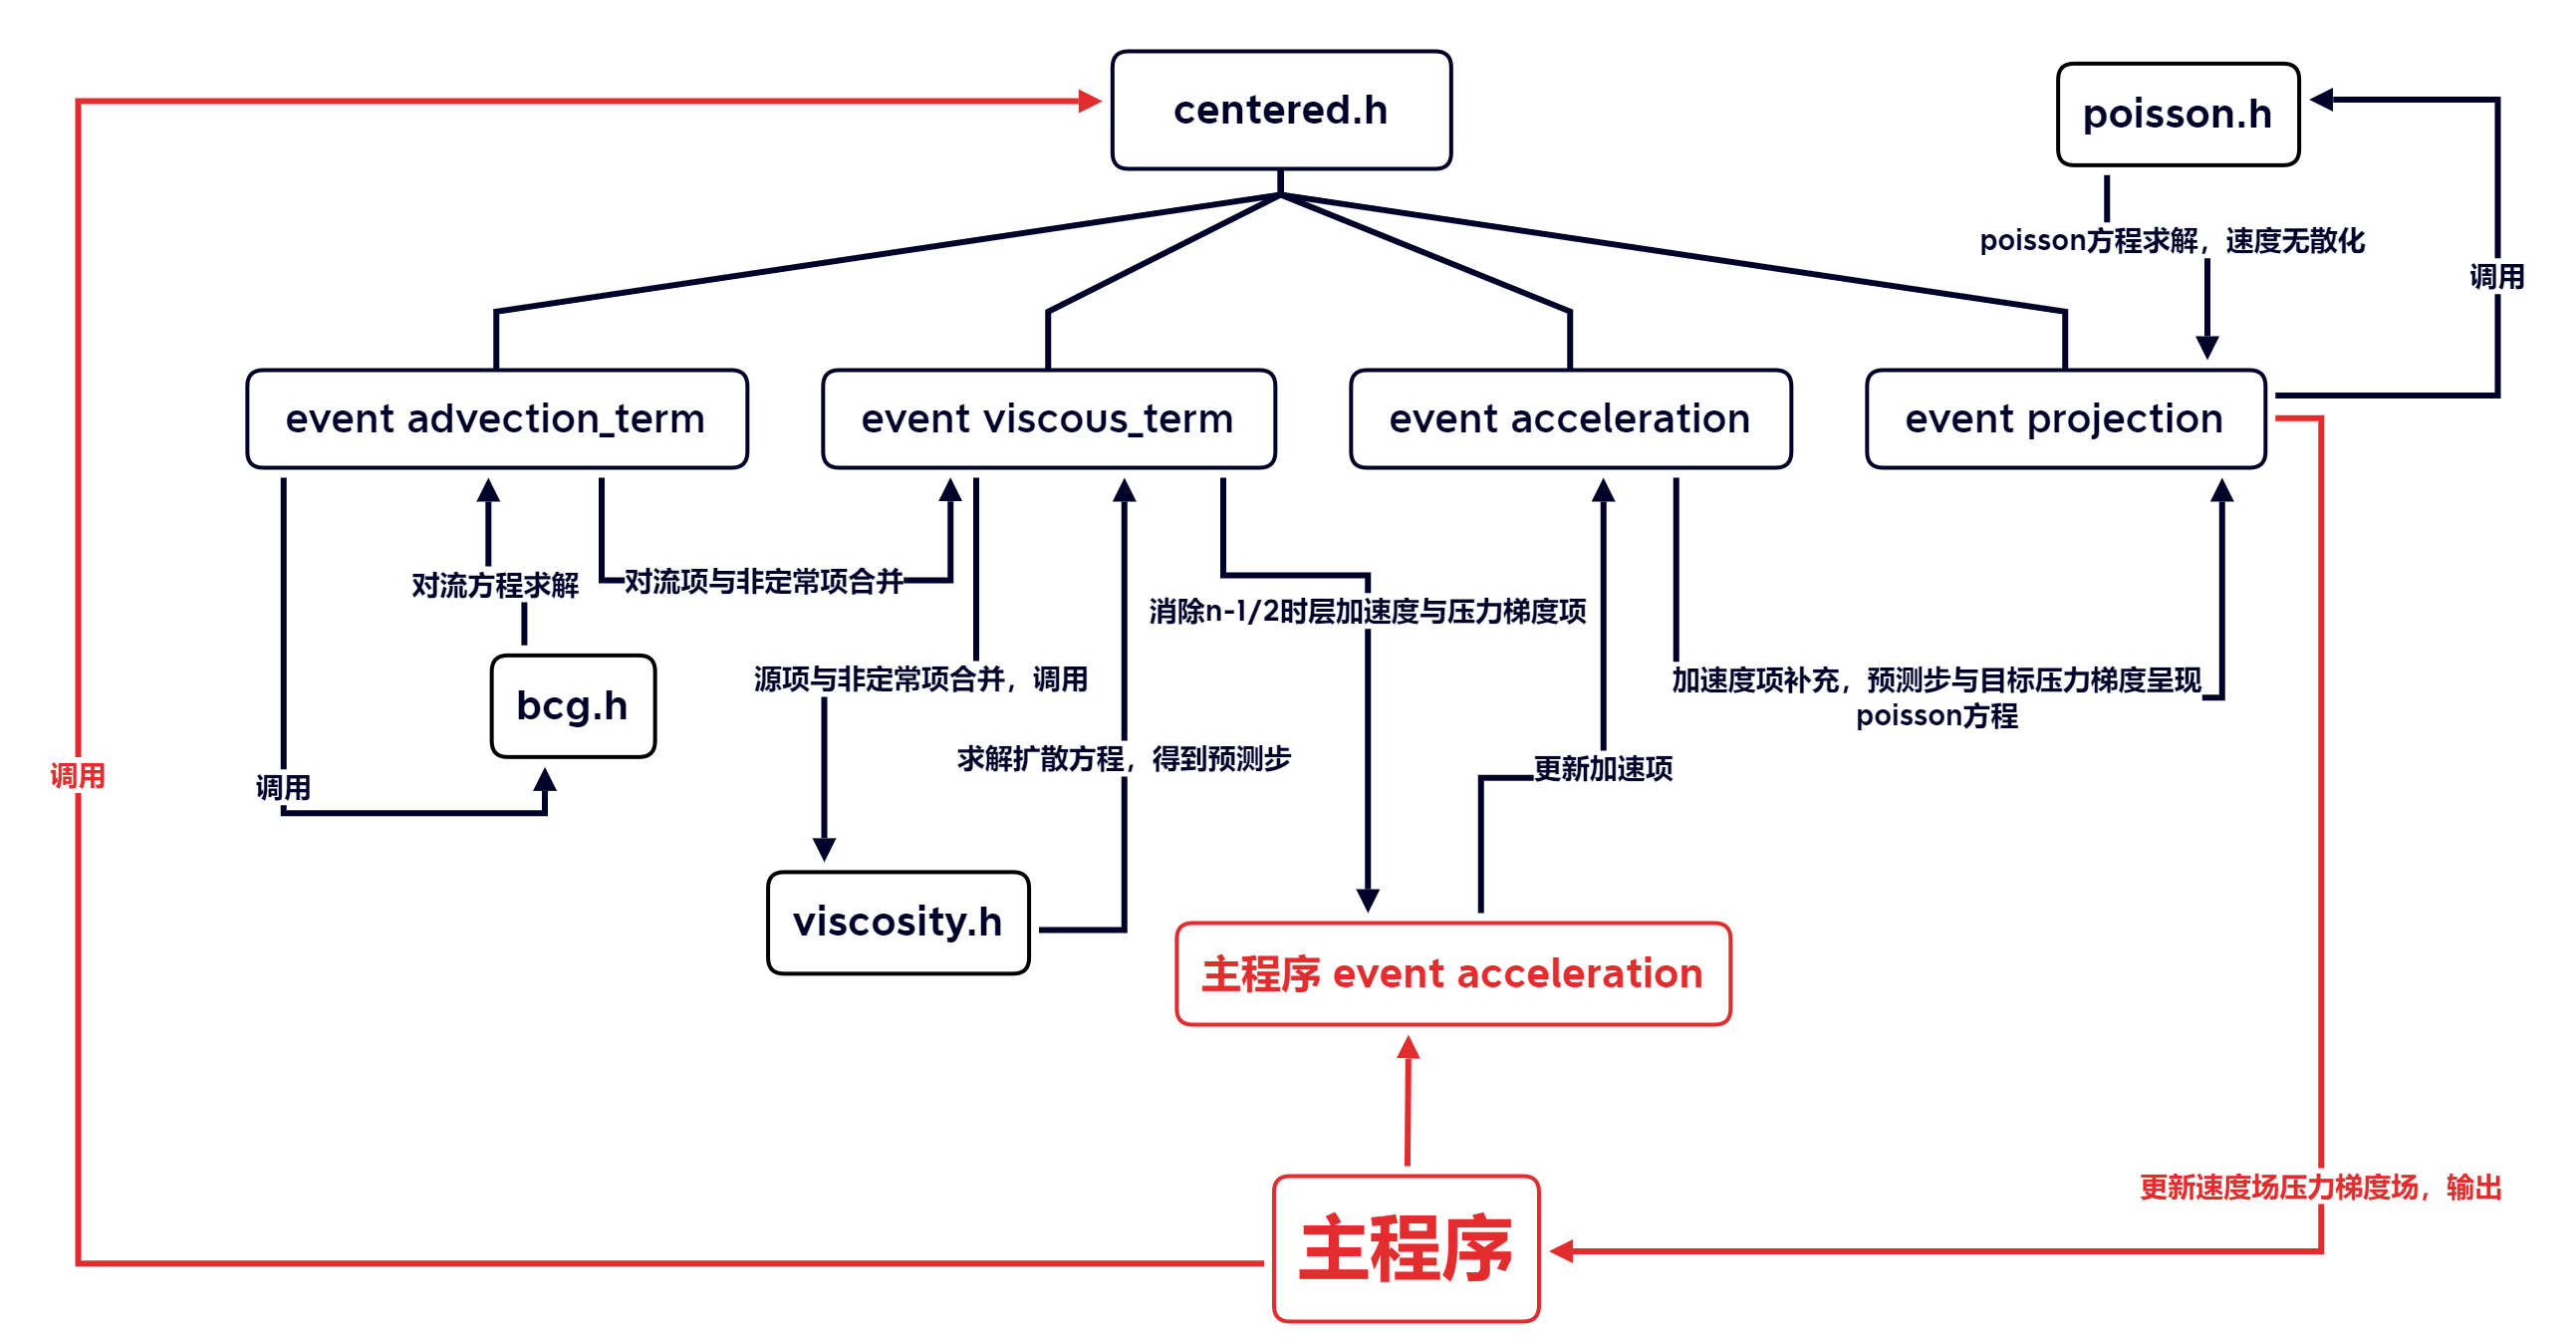
\includegraphics[width=1.0\textwidth]{centered.h.png}
  \caption{centered.h头文件中主要函数关系}
\end{figure}
\subsection{基础代码引用,边界条件设置,初始条件设置}\label{sec:fundemantel}
相关情况设置于注释中并不做太多解释。(embed边界的相关设置仍待查)
\begin{minted}[mathescape=true,breaklines]{lexer.py:DiffLexer -x}
#include "run.h"
#include "timestep.h"
#include "bcg.h"//注释:对流方程迭代计算
#if EMBED
# include "viscosity-embed.h"
#else
# include "viscosity.h"//注释:扩散方程迭代计算
#endif
/**
The primary variables are the centered pressure field $p$ and the
centered velocity field $\mathbf{u}$. The centered vector field
$\mathbf{g}$ will contain pressure gradients and acceleration terms.

We will also need an auxilliary face velocity field $\mathbf{u}_f$ and
the associated centered pressure field $p_f$. */

scalar p[];
vector u[], g[];
scalar pf[];
face vector uf[];

/**
In the case of variable density, the user will need to define both the
face and centered specific volume fields ($\alpha$ and $\alpha_c$
respectively) i.e. $1/\rho$. If not specified by the user, these
fields are set to one i.e. the density is unity.

Viscosity is set by defining the face dynamic viscosity $\mu$; default
is zero.

The face field $\mathbf{a}$ defines the acceleration term; default is
zero.

The statistics for the (multigrid) solution of the pressure Poisson
problems and implicit viscosity are stored in *mgp*, *mgpf*, *mgu* 
respectively. 

If *stokes* is set to *true*, the velocity advection term
$\nabla\cdot(\mathbf{u}\otimes\mathbf{u})$ is omitted. This is a
reference to [Stokes flows](http://en.wikipedia.org/wiki/Stokes_flow)
for which inertia is negligible compared to viscosity. */

(const) face vector mu = zerof, a = zerof, alpha = unityf;
(const) scalar rho = unity;
mgstats mgp, mgpf, mgu;
bool stokes = false;

/**
## Boundary conditions

For the default symmetric boundary conditions, we need to ensure that
the normal component of the velocity is zero after projection. This
means that, at the boundary, the acceleration $\mathbf{a}$ must be
balanced by the pressure gradient. Taking care of boundary orientation
and staggering of $\mathbf{a}$, this can be written */
//说明:如event acceleration 所示,uf中包含了a,因此需要在对uf^{n+1}校正时,需要对边界上的uf减去a的值(令\Delta p=a)以满足uf=0

#if EMBED
# define neumann_pressure(i) (alpha.n[i] ? a.n[i]*fm.n[i]/alpha.n[i] :	\
                  a.n[i]*rho[]/(cm[] + SEPS))
#else
# define neumann_pressure(i) (a.n[i]*fm.n[i]/alpha.n[i])
#endif

p[right] = neumann (neumann_pressure(ghost));
p[left]  = neumann (- neumann_pressure(0));

#if AXI
uf.n[bottom] = 0.;
uf.t[bottom] = dirichlet(0); // since uf is multiplied by the metric which
                             // is zero on the axis of symmetry
p[top]    = neumann (neumann_pressure(ghost));
#else // !AXI
#  if dimension > 1
p[top]    = neumann (neumann_pressure(ghost));
p[bottom] = neumann (- neumann_pressure(0));
#  endif
#  if dimension > 2
p[front]  = neumann (neumann_pressure(ghost));
p[back]   = neumann (- neumann_pressure(0));
#  endif
#endif // !AXI

/**
For [embedded boundaries on trees](/src/embed-tree.h), we need to
define the pressure gradient for prolongation of pressure close to
embedded boundaries. */

#if TREE && EMBED
void pressure_embed_gradient (Point point, scalar p, coord * g)
{
  foreach_dimension()
    g->x = rho[]/(cm[] + SEPS)*(a.x[] + a.x[1])/2.;
}
#endif // TREE && EMBED

/**
## Initial conditions */

event defaults (i = 0)
{

  CFL = 0.8;//注释:影响时间步长的选取

  /**
  The pressures are never dumped. */

  p.nodump = pf.nodump = true;
  
  /**
  The default density field is set to unity (times the metric). */

  if (alpha.x.i == unityf.x.i) {
    alpha = fm;
    rho = cm;
  }
  else if (!is_constant(alpha.x)) {
    face vector alphav = alpha;
    foreach_face()
      alphav.x[] = fm.x[];
  }

  /**
  On trees, refinement of the face-centered velocity field needs to
  preserve the divergence-free condition. */
//说明:对不同层级网格中变量和embed边界网格的插值,由细到粗或由粗到细

#if TREE
  uf.x.refine = refine_face_solenoidal;

  /**
  When using [embedded boundaries](/src/embed.h), the restriction and
  prolongation operators need to take the boundary into account. */

#if EMBED
  uf.x.refine = refine_face;
  foreach_dimension()
    uf.x.prolongation = refine_embed_face_x;
  for (scalar s in {p, pf, u, g}) {
    s.restriction = restriction_embed_linear;
    s.refine = s.prolongation = refine_embed_linear;
    s.depends = list_add (s.depends, cs);
  }
  for (scalar s in {p, pf})
    s.embed_gradient = pressure_embed_gradient;
#endif // EMBED
#endif // TREE
}


/**
We had some objects to display by default. */

event default_display (i = 0)
  display ("squares (color = 'u.x', spread = -1);");

/**
After user initialisation, we initialise the face velocity and fluid
properties. */

double dtmax;

event init (i = 0)
{
  trash ({uf});
  foreach_face()
    uf.x[] = fm.x[]*face_value (u.x, 0);

  /**
  We update fluid properties. */

  event ("properties");

  /**
  We set the initial timestep (this is useful only when restoring from
  a previous run). */

  dtmax = DT;
  event ("stability");
}

/**
## Time integration

The timestep for this iteration is controlled by the CFL condition,
applied to the face centered velocity field $\mathbf{u}_f$; and the
timing of upcoming events. */

event set_dtmax (i++,last) dtmax = DT;

event stability (i++,last) {
  dt = dtnext (stokes ? dtmax : timestep (uf, dtmax));//根据限制条件设置最大时间步
}

/**
If we are using VOF or diffuse tracers, we need to advance them (to
time $t+\Delta t/2$) here. Note that this assumes that tracer fields
are defined at time $t-\Delta t/2$ i.e. are lagging the
velocity/pressure fields by half a timestep. */
//说明:为了与u形成时间上的交错,初始各参数均被假定在-Delta t/2时刻,(p应该也应是被假定在-Delta t/2时刻?)

event vof (i++,last);
event tracer_advection (i++,last);
event tracer_diffusion (i++,last);

/**
The fluid properties such as specific volume (fields $\alpha$ and
$\alpha_c$) or dynamic viscosity (face field $\mu_f$) -- at time
$t+\Delta t/2$ -- can be defined by overloading this event. */

event properties (i++,last);

\end{minted}
\subsection{对流项处理及对流方程计算}\label{sec:advection}
在本小节中我们对对流项进行处理,用已知$\mathbf{u^n}$构建位于单元面上的面元速度$\mathbf{u_f^{n+\frac{1}{2}}}$,具体的推导公式在bcg.h中详细阐述,后使用在poisson.h文件中构建的projection函数对所求得$\mathbf{u_f^{n+\frac{1}{2}}}$进行无散化,再带入advection函数中求解方程\ref{equ:duiliu},从而与$\mathbf{u^n}$一同化为$\mathbf{u^{**}}$
\begin{minted}[mathescape=true,breaklines]{lexer.py:DiffLexer -x}
void prediction()
{
  vector du;
  foreach_dimension() {
    scalar s = new scalar;
    du.x = s;
  }

  if (u.x.gradient)
    foreach()
      foreach_dimension() {
#if EMBED
        if (!fs.x[] || !fs.x[1])
      du.x[] = 0.;
    else
#endif
      du.x[] = u.x.gradient (u.x[-1], u.x[], u.x[1])/Delta;//gradient是在common.h中保存的每个scalar都具有的数据结构特别类型
      }
  else
    foreach()
      foreach_dimension() {
#if EMBED
        if (!fs.x[] || !fs.x[1])
      du.x[] = 0.;
    else
#endif
      du.x[] = (u.x[1] - u.x[-1])/(2.*Delta);//其实就是求该方向上的梯度
    }

  trash ({uf});
  foreach_face() {
    double un = dt*(u.x[] + u.x[-1])/(2.*Delta), s = sign(un);
    int i = -(s + 1.)/2.;
    uf.x[] = u.x[i] + (g.x[] + g.x[-1])*dt/4. + s*(1. - s*un)*du.x[i]*Delta/2.;
    #if dimension > 1
    if (fm.y[i,0] && fm.y[i,1]) {
      double fyy = u.y[i] < 0. ? u.x[i,1] - u.x[i] : u.x[i] - u.x[i,-1];
      uf.x[] -= dt*u.y[i]*fyy/(2.*Delta);
    }
    #endif
    #if dimension > 2
    if (fm.z[i,0,0] && fm.z[i,0,1]) {
      double fzz = u.z[i] < 0. ? u.x[i,0,1] - u.x[i] : u.x[i] - u.x[i,0,-1];
      uf.x[] -= dt*u.z[i]*fzz/(2.*Delta);
    }
    #endif
    uf.x[] *= fm.x[];
  }

  delete ((scalar *){du});
}

/**
Advection term

We predict the face velocity field $\mathbf{u}_f$ at time $t+\Delta t/2$ then project it to make it divergence-free. We can then use it to
compute the velocity advection term, using the standard
Bell-Collela-Glaz advection scheme for each component of the velocity
field. */

event advection_term (i++,last)
{
  if (!stokes) {
    prediction();//注释:预测步,uf位于n+1/2时层
    mgpf = project (uf, pf, alpha, dt/2., mgpf.nrelax);//注释:uf无散化,pf位于n+1/2时层
    advection ((scalar *){u}, uf, dt, (scalar *){g});//注释:对流方程计算得到$\mathbf{u^{**}}$
  }
}
\end{minted}

\subsection{扩散项处理}\label{sec:diffusion}
在得到$\mathbf{u^{**}}$后我们将$\nabla p^{n-\frac{1}{2}}$以及加速度表面张力项等汇入$\mathbf{u^{**}}$见公式\ref{equ:yuanxiangjiazai}
\begin{minted}[mathescape=true,breaklines]{lexer.py:DiffLexer -x}
/**
### Viscous term

We first define a function which adds the pressure gradient and
acceleration terms. */

static void correction (double dt)
{
  foreach()
    foreach_dimension()
      u.x[] += dt*g.x[];
}

/**
The viscous term is computed implicitly. We first add the pressure
gradient and acceleration terms, as computed at time $t$, then call
the implicit viscosity solver. We then remove the acceleration and
pressure gradient terms as they will be replaced by their values at
time $t+\Delta t$. */

event viscous_term (i++,last)
{
  if (constant(mu.x) != 0.) {
    correction (dt);//构造poisson型方程的残差,直接构造$\mathbf{u^{***}}$
    mgu = viscosity (u, mu, rho, dt, mgu.nrelax);
    correction (-dt);//注意此时由于viscosity的计算u[]已经存储的是$\mathbf{u^*}$,让其减去位于$n-\frac{1}{2}$的加速度项与压力梯度项
  }

  /**
  We reset the acceleration field (if it is not a constant). */

  if (!is_constant(a.x)) {
    face vector af = a;
    trash ({af});
    foreach_face()
      af.x[] = 0.;//刷新加速度项
  }
}
\end{minted}

通过操作
\mintinline{lexer.py:DiffLexer -x}{mgu = viscosity (u, mu, rho, dt, mgu.nrelax);}
解方程\ref{equ:kuosan}。\par
由此我们得解$\mathbf{u^{*}}$并在\mintinline{lexer.py:DiffLexer -x}{correction (-dt);}中对其做$\mathbf{u^*}+\frac{\Delta t}{\rho_{n+\frac{1}{2}}}(\nabla p^{n-\frac{1}{2}}-\mathbf{a}^{n-\frac{1}{2}})$

\subsection{速度修正项}\label{sec:projection}
由于加速项为面元,而求得的$\mathbf{u^{*}}$为体元项,为了poisson方程求解方便,我们将所得速度项向单元面上插值,并更新补充$n+\frac{1}{2}$的加速度项(如方程\ref{equ:sudugengxin},关于加速度项更新详见第\ref{sec:fuluA}节附录),则此时$\mathbf{u^*_{f\ new}}$满足

\begin{equation}
    \mathbf{u_f^{n+1}} = \mathbf{u^*_{f\ new}}-\frac{\Delta t}{\rho_{n+\frac{1}{2}}}\nabla p_{n+\frac{1}{2}}
\end{equation}
即带入poisson求解器再进行求解,同时更新压力项$p^{n+\frac{1}{2}}$
\begin{minted}[mathescape=true,breaklines]{lexer.py:DiffLexer -x}
/**
### Acceleration term

The acceleration term $\mathbf{a}$ needs careful treatment as many
equilibrium solutions depend on exact balance between the acceleration
term and the pressure gradient: for example Laplace's balance for
surface tension or hydrostatic pressure in the presence of gravity.

To ensure a consistent discretisation, the acceleration term is
defined on faces as are pressure gradients and the centered combined
acceleration and pressure gradient term $\mathbf{g}$ is obtained by
averaging. 

The (provisionary) face velocity field at time $t+\Delta t$ is
obtained by interpolation from the centered velocity field. The
acceleration term is added. */
//说明:基于balance-force方法,压力和表面张力两项在程序各方程中同时考虑。

event acceleration (i++,last)
{
  trash ({uf});
  foreach_face()
    uf.x[] = fm.x[]*(face_value (u.x, 0) + dt*a.x[]);//此处为更新位于$n+\frac{1}{2}$时层的加速度项,并将其作为补充,填充速度项,从而获得速度预测步与压力梯度的poisson方程
}

/**
## Approximate projection

This function constructs the centered pressure gradient and
acceleration field *g* using the face-centered acceleration field *a*
and the cell-centered pressure field *p*. */

void centered_gradient (scalar p, vector g)
{

  /**
  We first compute a face field $\mathbf{g}_f$ combining both
  acceleration and pressure gradient. */

  face vector gf[];
  foreach_face()
    gf.x[] = fm.x[]*a.x[] - alpha.x[]*(p[] - p[-1])/Delta;

  /**
  We average these face values to obtain the centered, combined
  acceleration and pressure gradient field. */

  trash ({g});
  foreach()
    foreach_dimension()
      g.x[] = (gf.x[] + gf.x[1])/(fm.x[] + fm.x[1] + SEPS);
}

/**
To get the pressure field at time $t + \Delta t$ we project the face
velocity field (which will also be used for tracer advection at the
next timestep). Then compute the centered gradient field *g*. */

event projection (i++,last)
{
  mgp = project (uf, p, alpha, dt, mgp.nrelax);
  centered_gradient (p, g);

  /**
  We add the gradient field *g* to the centered velocity field. */

  correction (dt);//此处是对网格中心速度场进行源项附加(注意之前加速度操作及压力梯度更新都是面元速度,单元中心速度自扩散项中去掉$n-\frac{1}{2}$时层的加速度与压力梯度后再未更新)
}

/**
Some derived solvers need to hook themselves at the end of the
timestep. */

event end_timestep (i++, last);

/**
## Adaptivity

After mesh adaptation fluid properties need to be updated. When using
[embedded boundaries](/src/embed.h) the fluid fractions and face
fluxes need to be checked for inconsistencies. */

#if TREE
event adapt (i++,last) {
#if EMBED
  fractions_cleanup (cs, fs);
  foreach_face()
    if (uf.x[] && !fs.x[])
      uf.x[] = 0.;
#endif
  event ("properties");
}
#endif
\end{minted}
最后将所有数据进行更新,一个时层的NS方程即求解完毕。
\section{附录A:Basilisk中event的执行顺序与特殊数据结构的赋值}\label{sec:fuluA}

centered.h中加速度项的更新并没有在程序中明示,实际上的更新发生在调用centered.h头文件的主程序中,以Basilisk官网中的Bubble rising in a large tank为例\url{http://basilisk.fr/src/examples/bubble.c},可以发现主程序部分中,有与centered.h头文件中同名的event acceleration:
\begin{minted}[mathescape=true,breaklines]{lexer.py:DiffLexer -x}
event acceleration (i++) {
  face vector av = a;
  foreach_face(y)
    av.y[] -= 1.;
}
\end{minted}
此处也正是整体算法中,加速度更新的操作;下面从两个方向分析该代码
\subsection{event执行顺序}
基于官网$Basilisk C$ \url{http://basilisk.fr/Basilisk%20C#event-inheritance}中的相关介绍以及代码实验,现对Basilisk中同名event的继承执行顺序进行概述\par
\begin{enumerate}
    \item 程序进行编译运行时所有的头文件将会被直接复制打开,所有同名的event视为一组(group)将会被同时执行,其相较于其他名称event被执行顺序取决于该组event中最先出现的那一个的位置
    \item 组内event的执行顺序和出现顺序\textcolor{red}{相反},即最先执行在源程序中出现最晚的event
\end{enumerate}
为了测试event执行顺序编写以下主程序及头文件\par
主程序示例:
\begin{minted}[mathescape=true,breaklines]{lexer.py:DiffLexer -x}
#include "eventtest1.h"
//#include "eventtest2.h"
#include "run.h"

#define MAXTIME 1



int main()
{
  run();
}

event scriptA(i=0; i<=MAXTIME; i++)
{
  fprintf(stdout,"script1\n");
}

event scriptB(i=0; i<=MAXTIME; i++)
{
  fprintf(stdout,"script2\n");
}
\end{minted}
头文件示例:
\begin{minted}[mathescape=true,breaklines]{lexer.py:DiffLexer -x}
event test1A(i++,last)
{
  fprintf(stdout,"test1A\n");
}

event scriptA(i++,last)
{
  fprintf(stdout,"test1B\n");
}
\end{minted}
由上述规则可知,在运行Bubble.c时,主程序中名为acceleration的event会率先被忽略,而在头文件中同名event执行时被唤醒,并首先执行主程序acceleration编写内容,再执行头文件中的acceleration。
\subsection{特殊数据结构的赋值}
在主程序的acceleration中有操作\mintinline{lexer.py:DiffLexer -x}{face vector av = a;},这里并不是赋值操作,而是指针地址传递,其中\mintinline{lexer.py:DiffLexer -x}{av,a}均为\mintinline{lexer.py:DiffLexer -x}{face vector*}故我们在之后对\mintinline{lexer.py:DiffLexer -x}{av}进行的任何操作,其实质上都是在对\mintinline{lexer.py:DiffLexer -x}{a}进行各种同等操作。\par
类似的,所有Basilisk自带的数据结构,直接对名称使用等于号,都是对内存地址进行传递,而并非赋值。
\section{附录B:标准Fractional Step Method算法及误差}
在前文中提到,centered.h\textbf{大体上}运用了FSM方法,而其不同之处便在于扩散项的离散,标准方法的离散为:
 \begin{equation}\label{equ:fsm}
    \rho_{n+\frac{1}{2}}\frac{\mathbf{u}^* - \mathbf{u}^{***}}{\Delta t}= \nabla \cdot [\mu^{n+\frac{1}{2}}(\mathbf{D^*}+\mathbf{D^{n}})]
\end{equation}
而误差为:
\begin{equation}
    \epsilon = \frac{1}{2}(\Delta t)^2\mathbf{L}(\frac{1}{\rho}\mathbf{G}(\frac{\partial p}{\partial t}))
\end{equation}
\printbibliography[heading=bibintoc, title=\ebibname]
\end{document}
